\section{Second Member}
This is the section dedicated to one of the team members, and it should be written individually . It can include a range of things; first subsection is a space for you to point out the strengths and weaknesses of the module, including complaints about the module coordinator Max Wilson. The second section should have a selfie image with Max! The last part of it is the most important one. You will need to write a paragraph about what you have learned in this module. You can write it in \textbf{Bold} if you want or you can use other fonts. 

Please do not forget:
\begin{itemize}
	\item First paragraph should have your comments about the module
	\item Second one, a selfie img with Max
	\item Last one, what you learned in this module.
\end{itemize}

\subsection{Comments about the module}
This is the first subsection. Do not forget to include the best parts about the module as well as what you did not like about Max Wilson during the term.
The FSE module has been very enjoyable. Despite me hearing that other students think it is the most boring module in terms of content, I do find some of it quite interesting, and the presentations from Max are well made and thought out. However, one thing I am not a fan of is the large number of expected reading set for the module. It's difficult to know what will important in the exam when given 5 pages of dense text in a pdf to read after every lecture.

\subsection{Selfie with Max}
Below is a selfie of me and Max Wilson
\begin{figure}[h]
\caption{Selfie with Max}
\centering
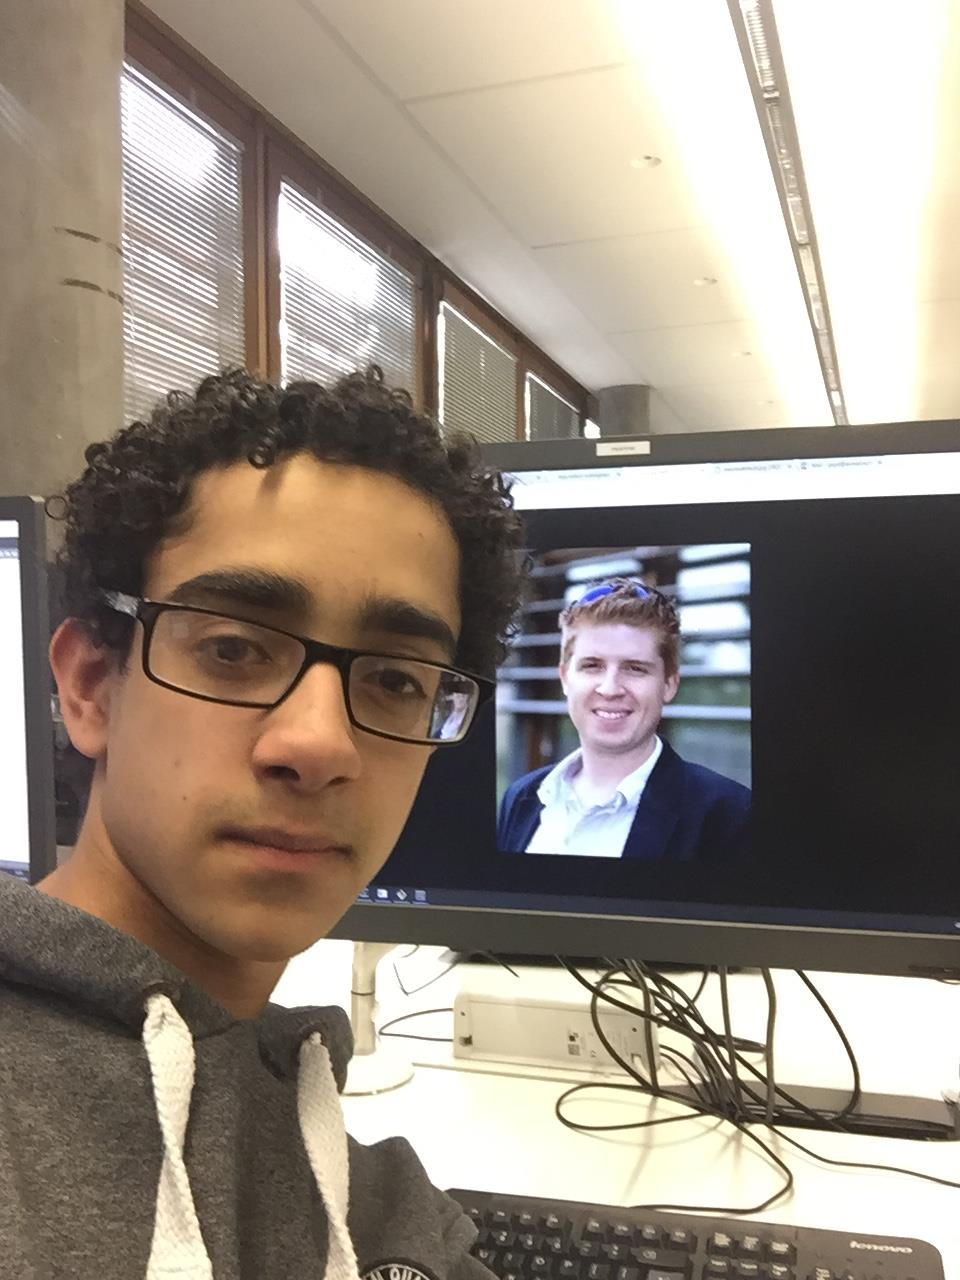
\includegraphics[width=0.5\textwidth]{psyit_real_selfie}
\label{fig:selfie}
\end{figure}

You can then use the label of the figure to reference it later with the command ${\backslash}ref.$ you can comment out the next line to see an example of how it works.

% My selfie with Max is in  Figure~\ref{fig:selfie}.

\subsection{What I have learned in this module}
In this module I have learnt about the various stages in the software engineering process as well as the different methodologies and strategies involved in creating successful software as a team.

Although we haven't done any real coding as teams as of yet, I have learnt a lot about how to work as team through the weekly lab sessions.

